\chapter{Conception et architecture de la plateforme}

Les besoins spécifiés au chapitre 2 et les méthodes de risque présentées aux chapitres 3 et 4 doivent maintenant se traduire en une architecture logicielle capable de les mettre en œuvre. Ce chapitre présente cette architecture à plusieurs niveaux, globale, logique puis physique, avant de la détailler par des diagrammes UML qui formalisent les interactions entre composants. Il se referme sur l'architecture propre à l'assistant conversationnel, qui s'appuie sur ce même socle sans s'y substituer. Le chapitre suivant présente la réalisation effective de cette architecture et sa validation.

\section{Architecture globale de la plateforme}

Les deux volets de la plateforme présentés au chapitre 1, l'Origination et le suivi de portefeuille, se traduisent architecturalement par deux chemins de traitement distincts. Les traitements \emph{batch} regroupent, d'une part, l'entraînement et la sauvegarde des modèles présentés au chapitre 3 et, d'autre part, leur utilisation pour calculer, à l'échelle du portefeuille, les indicateurs de risque, de capital et de rentabilité présentés au chapitre 4 ; ces deux opérations sont distinctes, la seconde se contentant de charger les modèles déjà entraînés par la première. Un chemin temps réel évalue, à l'unité, une nouvelle demande de crédit soumise via l'interface web.

Ces deux chemins réutilisent plusieurs moteurs de calcul communs, probabilité de défaut, perte en cas de défaut, exposition au défaut, détection de dégradation du risque, rentabilité et interprétabilité SHAP, mais pas nécessairement les mêmes instances entraînées : l'Origination s'appuie sur des modèles de probabilité de défaut entraînés spécifiquement pour l'évaluation d'une nouvelle demande, distincts de ceux présentés au chapitre 3 pour le suivi de portefeuille. Le moteur de décision, au sens de l'enchaînement complet présenté en section~4.5, n'est à ce jour effectivement exécuté que dans le chemin temps réel ; le moteur de décision dédié au suivi de portefeuille existe dans le code, mais n'est pas mobilisé dans le parcours de traitement actuellement exécuté. D'autres moteurs, enfin, n'interviennent que dans le suivi de portefeuille, notamment le modèle de survie utilisé pour la PD à horizon de vie résiduelle et la simulation Monte Carlo du capital de portefeuille, tous deux présentés au chapitre 4.

L'ensemble de ces traitements s'appuie sur une base de données PostgreSQL unique, organisée en six schémas distincts : les données entrantes, le Feature Store utilisé pour la modélisation, les résultats produits par les moteurs de risque, les éléments de gouvernance et de traçabilité, les vues consommées par les tableaux de bord, et les éléments d'authentification des utilisateurs, appliqués séparément au démarrage du backend. Cette base constitue un support de données commun aux deux chemins : le traitement batch y dépose les données et les résultats nécessaires au suivi du portefeuille, tandis que le chemin temps réel y accède pour consulter ou enregistrer les informations relatives aux demandes de crédit. Les modèles entraînés, quant à eux, sont chargés depuis leurs artefacts sauvegardés sur disque, jamais depuis cette base.

Au-dessus de cette base, un backend expose les traitements de la plateforme sous forme d'une API, consommée par une application web qui constitue l'unique point d'accès des utilisateurs, chacun selon les droits associés à son rôle, présentés au chapitre 2. Un assistant conversationnel complète cet ensemble de façon transversale : il interagit avec les données et les services de la plateforme, dans les limites des droits associés au rôle de l'utilisateur, afin de répondre à ses questions, mais n'intervient dans aucune décision de crédit, une limite imposée par le code lui-même et non seulement documentée ; son architecture propre est détaillée en section~5.5.

La figure~\ref{fig:flux-donnees} synthétise ces deux chemins sous la forme d'un flux de données global, des sources réelles jusqu'aux pages consultées par les utilisateurs, en marquant explicitement l'absence de transfert automatique entre les décisions individuelles d'Origination et le suivi de portefeuille : les deux chemins restent distincts jusque dans leurs résultats persistés.

\begin{figure}[htbp]
    \centering
    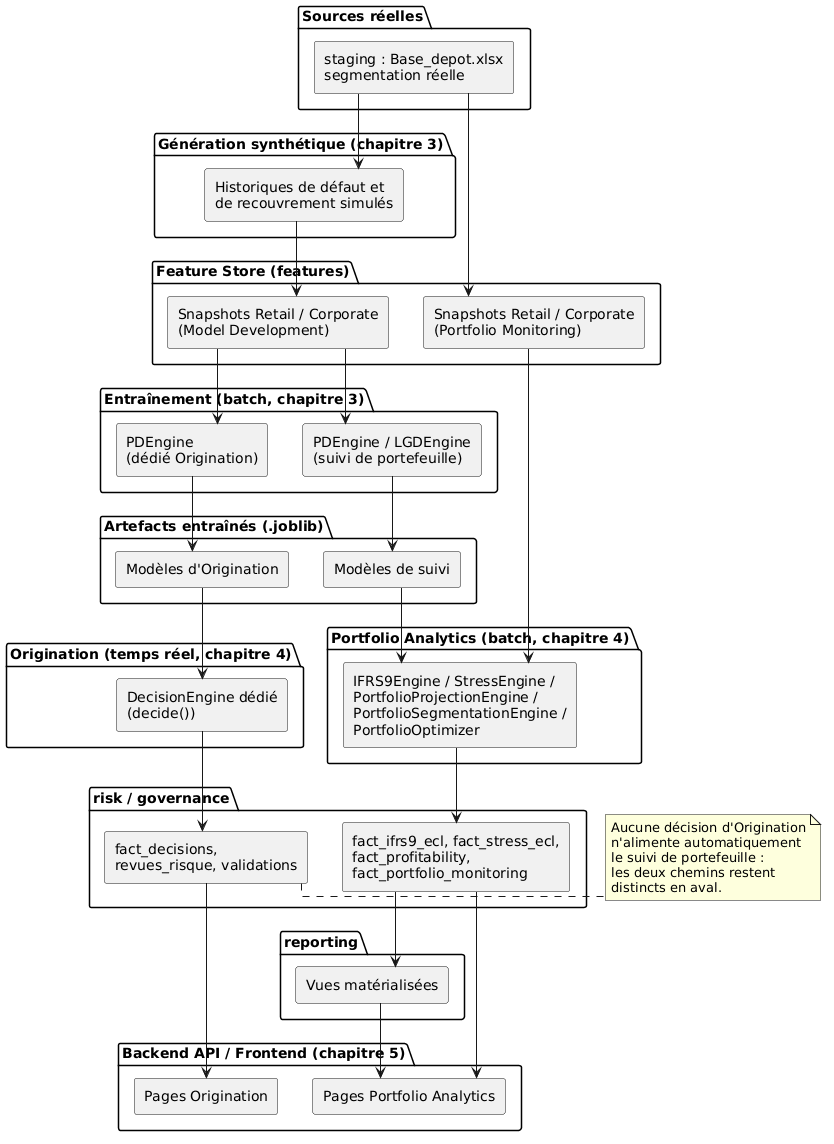
\includegraphics[width=\textwidth,height=0.85\textheight,keepaspectratio]{figures/flux_donnees_global.png}
    \caption{Flux de données global de la plateforme (élaboration personnelle).}
    \label{fig:flux-donnees}
\end{figure}

\section{Architecture logique}

La figure~\ref{fig:architecture-logique} présente l'organisation fonctionnelle de la plateforme, indépendamment de sa réalisation technique.

\begin{figure}[htbp]
    \centering
    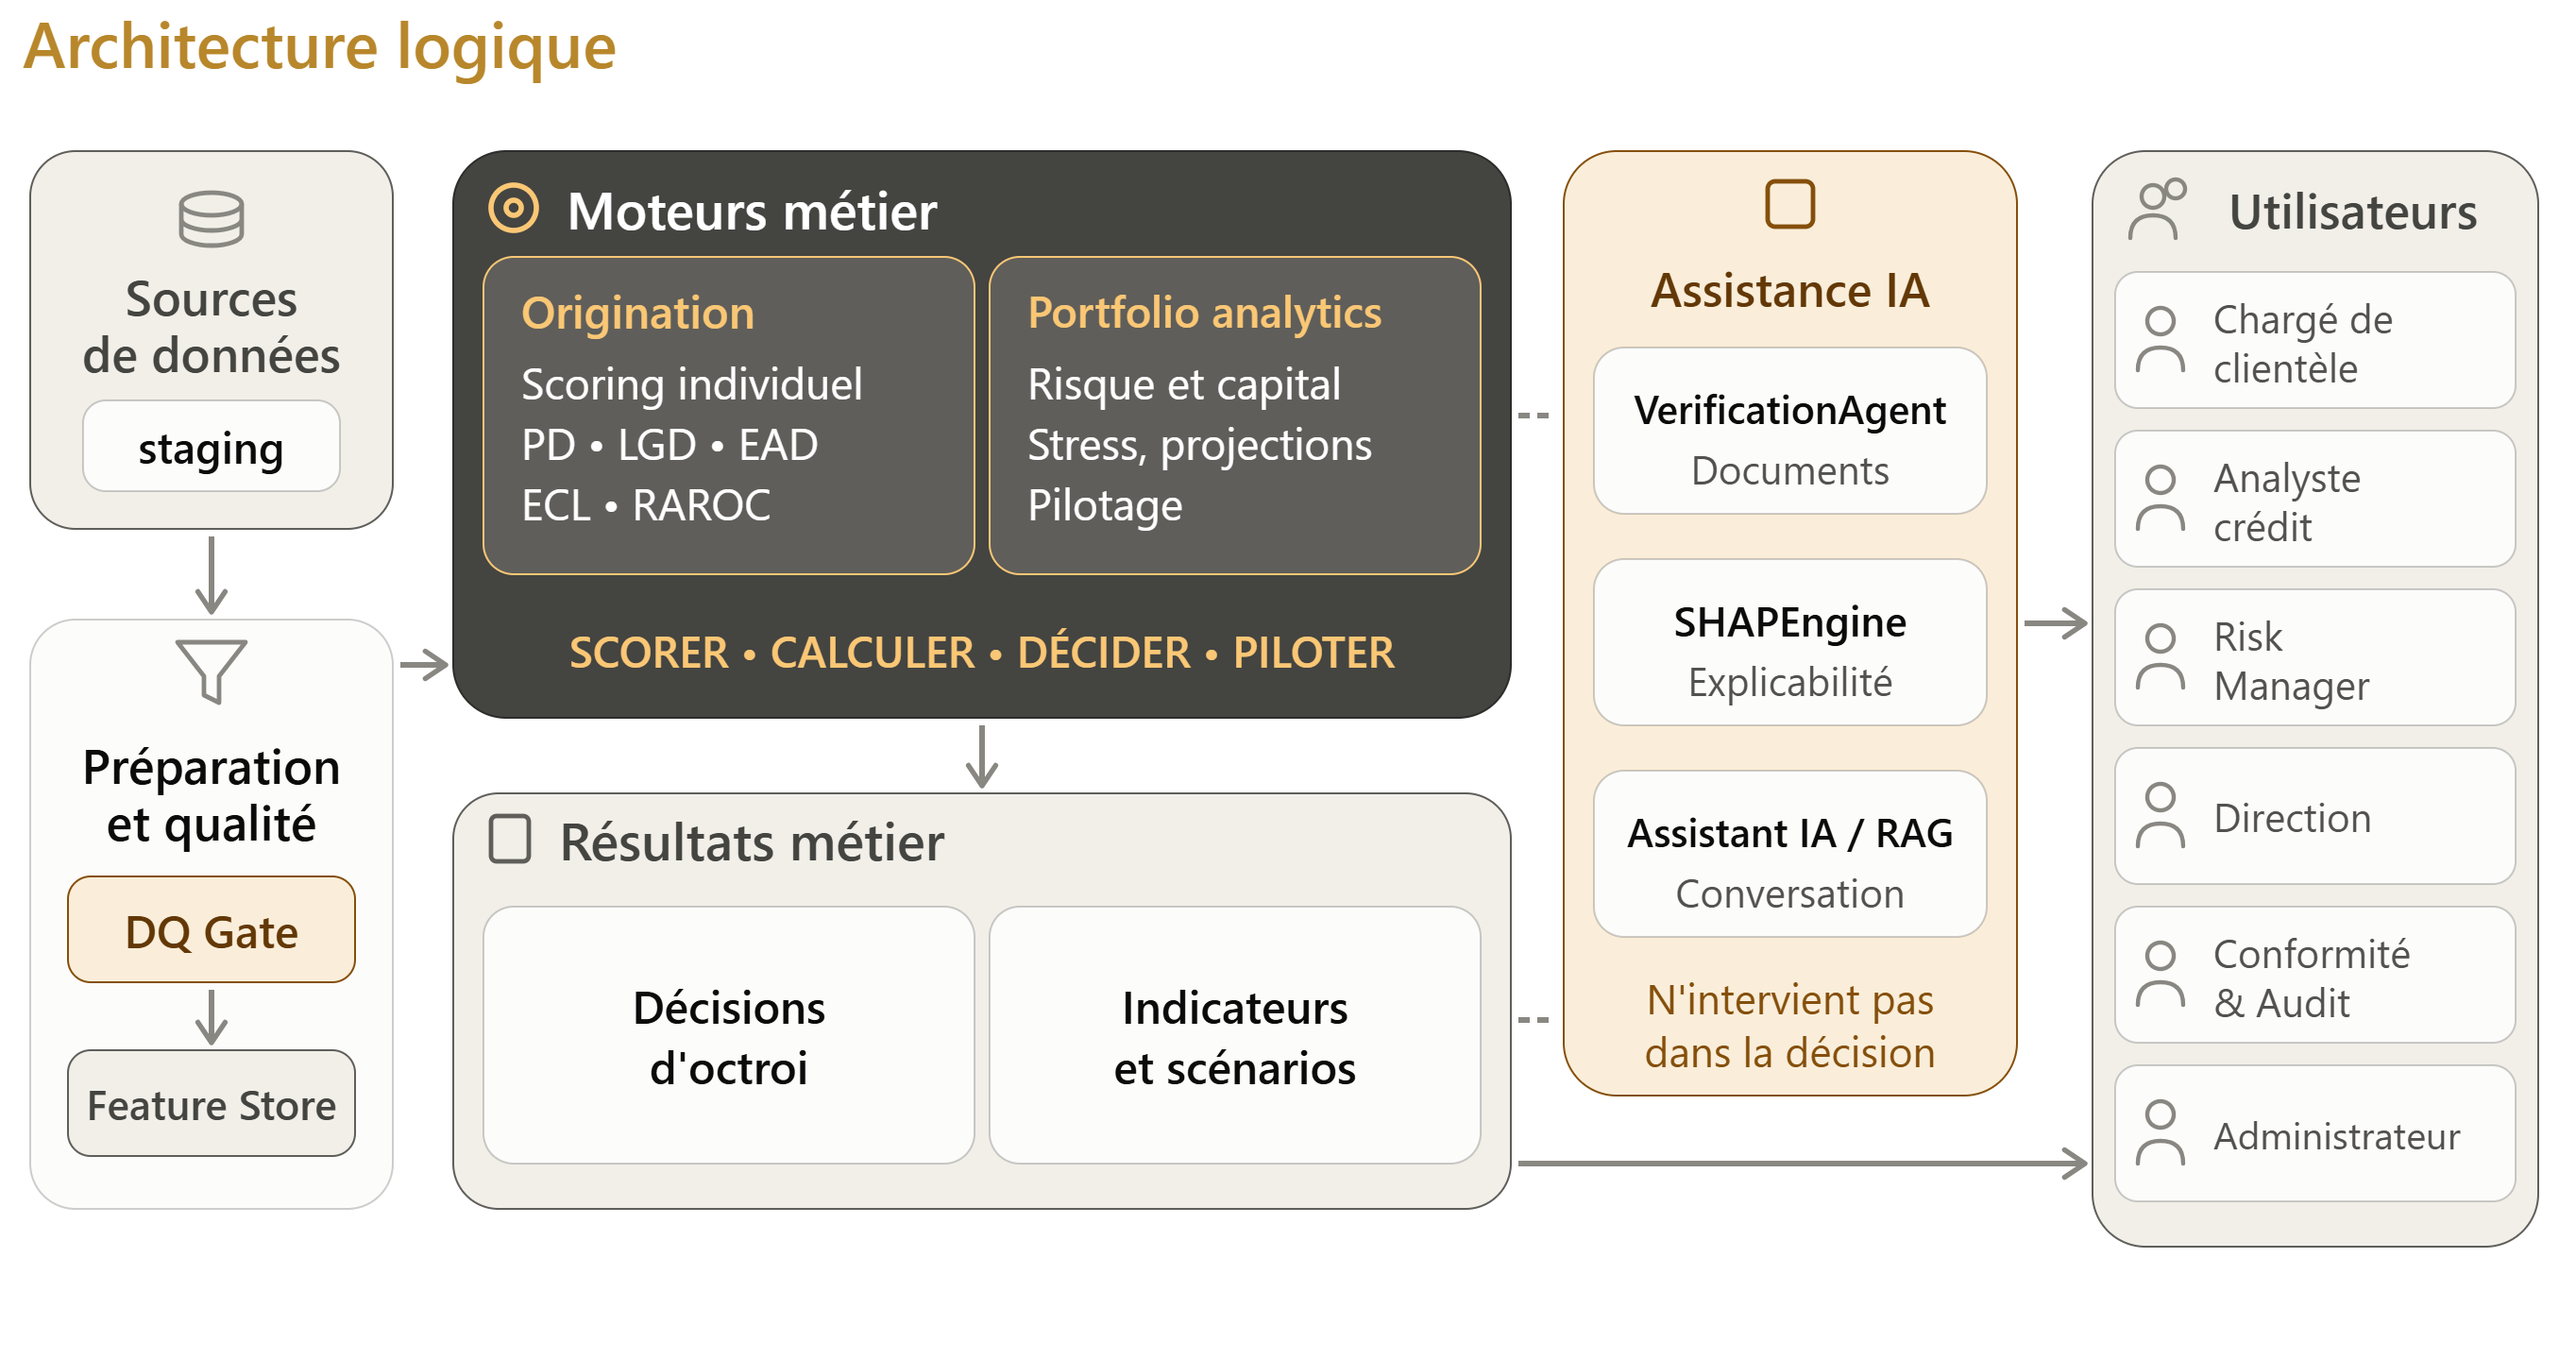
\includegraphics[width=\textwidth]{figures/architecture_logique.png}
    \caption{Architecture logique de la plateforme (élaboration personnelle).}
    \label{fig:architecture-logique}
\end{figure}

Les données réelles entrantes, principalement constituées des informations relatives aux clients et à leurs comptes, sont issues du schéma \texttt{staging} présenté au chapitre 3. Elles sont complétées, dans le cadre du projet, par les historiques de crédit et de remboursement synthétiques construits pour les besoins de la modélisation, également présentés au chapitre 3. L'ensemble est d'abord soumis à une étape de préparation et de qualité : un contrôle de qualité des données, une transformation, puis une construction du Feature Store qui alimente la modélisation.

Les moteurs métier exploitent les données préparées selon les besoins propres à chacun des deux volets déjà distingués au chapitre 1, plutôt qu'une alimentation identique. Pour le suivi de portefeuille, le Feature Store ci-dessus alimente les traitements batch et les modèles entraînés à partir des historiques disponibles : le parcours Portfolio Analytics mobilise ces données et ces modèles pour produire les indicateurs de risque, les pertes attendues, le capital économique et les mesures de rentabilité présentés aux chapitres 3 et 4. Pour l'Origination, les caractéristiques nécessaires à l'évaluation d'un dossier sont constituées séparément, à partir des informations du dossier et de l'historique client exploitable, pour alimenter une évaluation individuelle, probabilité de défaut, perte en cas de défaut, exposition au défaut, perte attendue et capital forfaitaire, rentabilité, puis les règles de décision présentées en section~4.5. Ces traitements produisent des résultats distincts selon le volet : une recommandation d'octroi, éventuellement assortie de conditions ou orientée vers une revue manuelle, accompagnée de son explication pour l'Origination ; des snapshots de risque, des indicateurs et des scénarios, des résultats de pilotage pour le suivi de portefeuille.

Des mécanismes d'explicabilité et de contrôle complètent ces traitements métier sans s'y substituer : l'interprétabilité SHAP contribue à l'explication des résultats de l'Origination, tandis que la vérification documentaire et l'orientation vers une revue humaine apportent des contrôles complémentaires au même parcours. L'assistant conversationnel, présenté en section~5.5, constitue pour sa part une couche consultative transversale : il permet aux utilisateurs d'interroger les données et les services de la plateforme, sans jamais intervenir dans une décision de crédit. Enfin, l'accès à ces résultats est soumis au contrôle d'accès par rôle présenté au chapitre 2, chaque acteur de la plateforme, chargé de clientèle, analyste crédit, Risk Manager, Direction, Conformité et Audit, Administrateur, ne consultant que ce que ses droits lui permettent.

\section{Architecture physique}

La figure~\ref{fig:architecture-physique} détaille la réalisation technique de cette organisation logique, dans l'environnement de développement local du projet.

\begin{figure}[htbp]
    \centering
    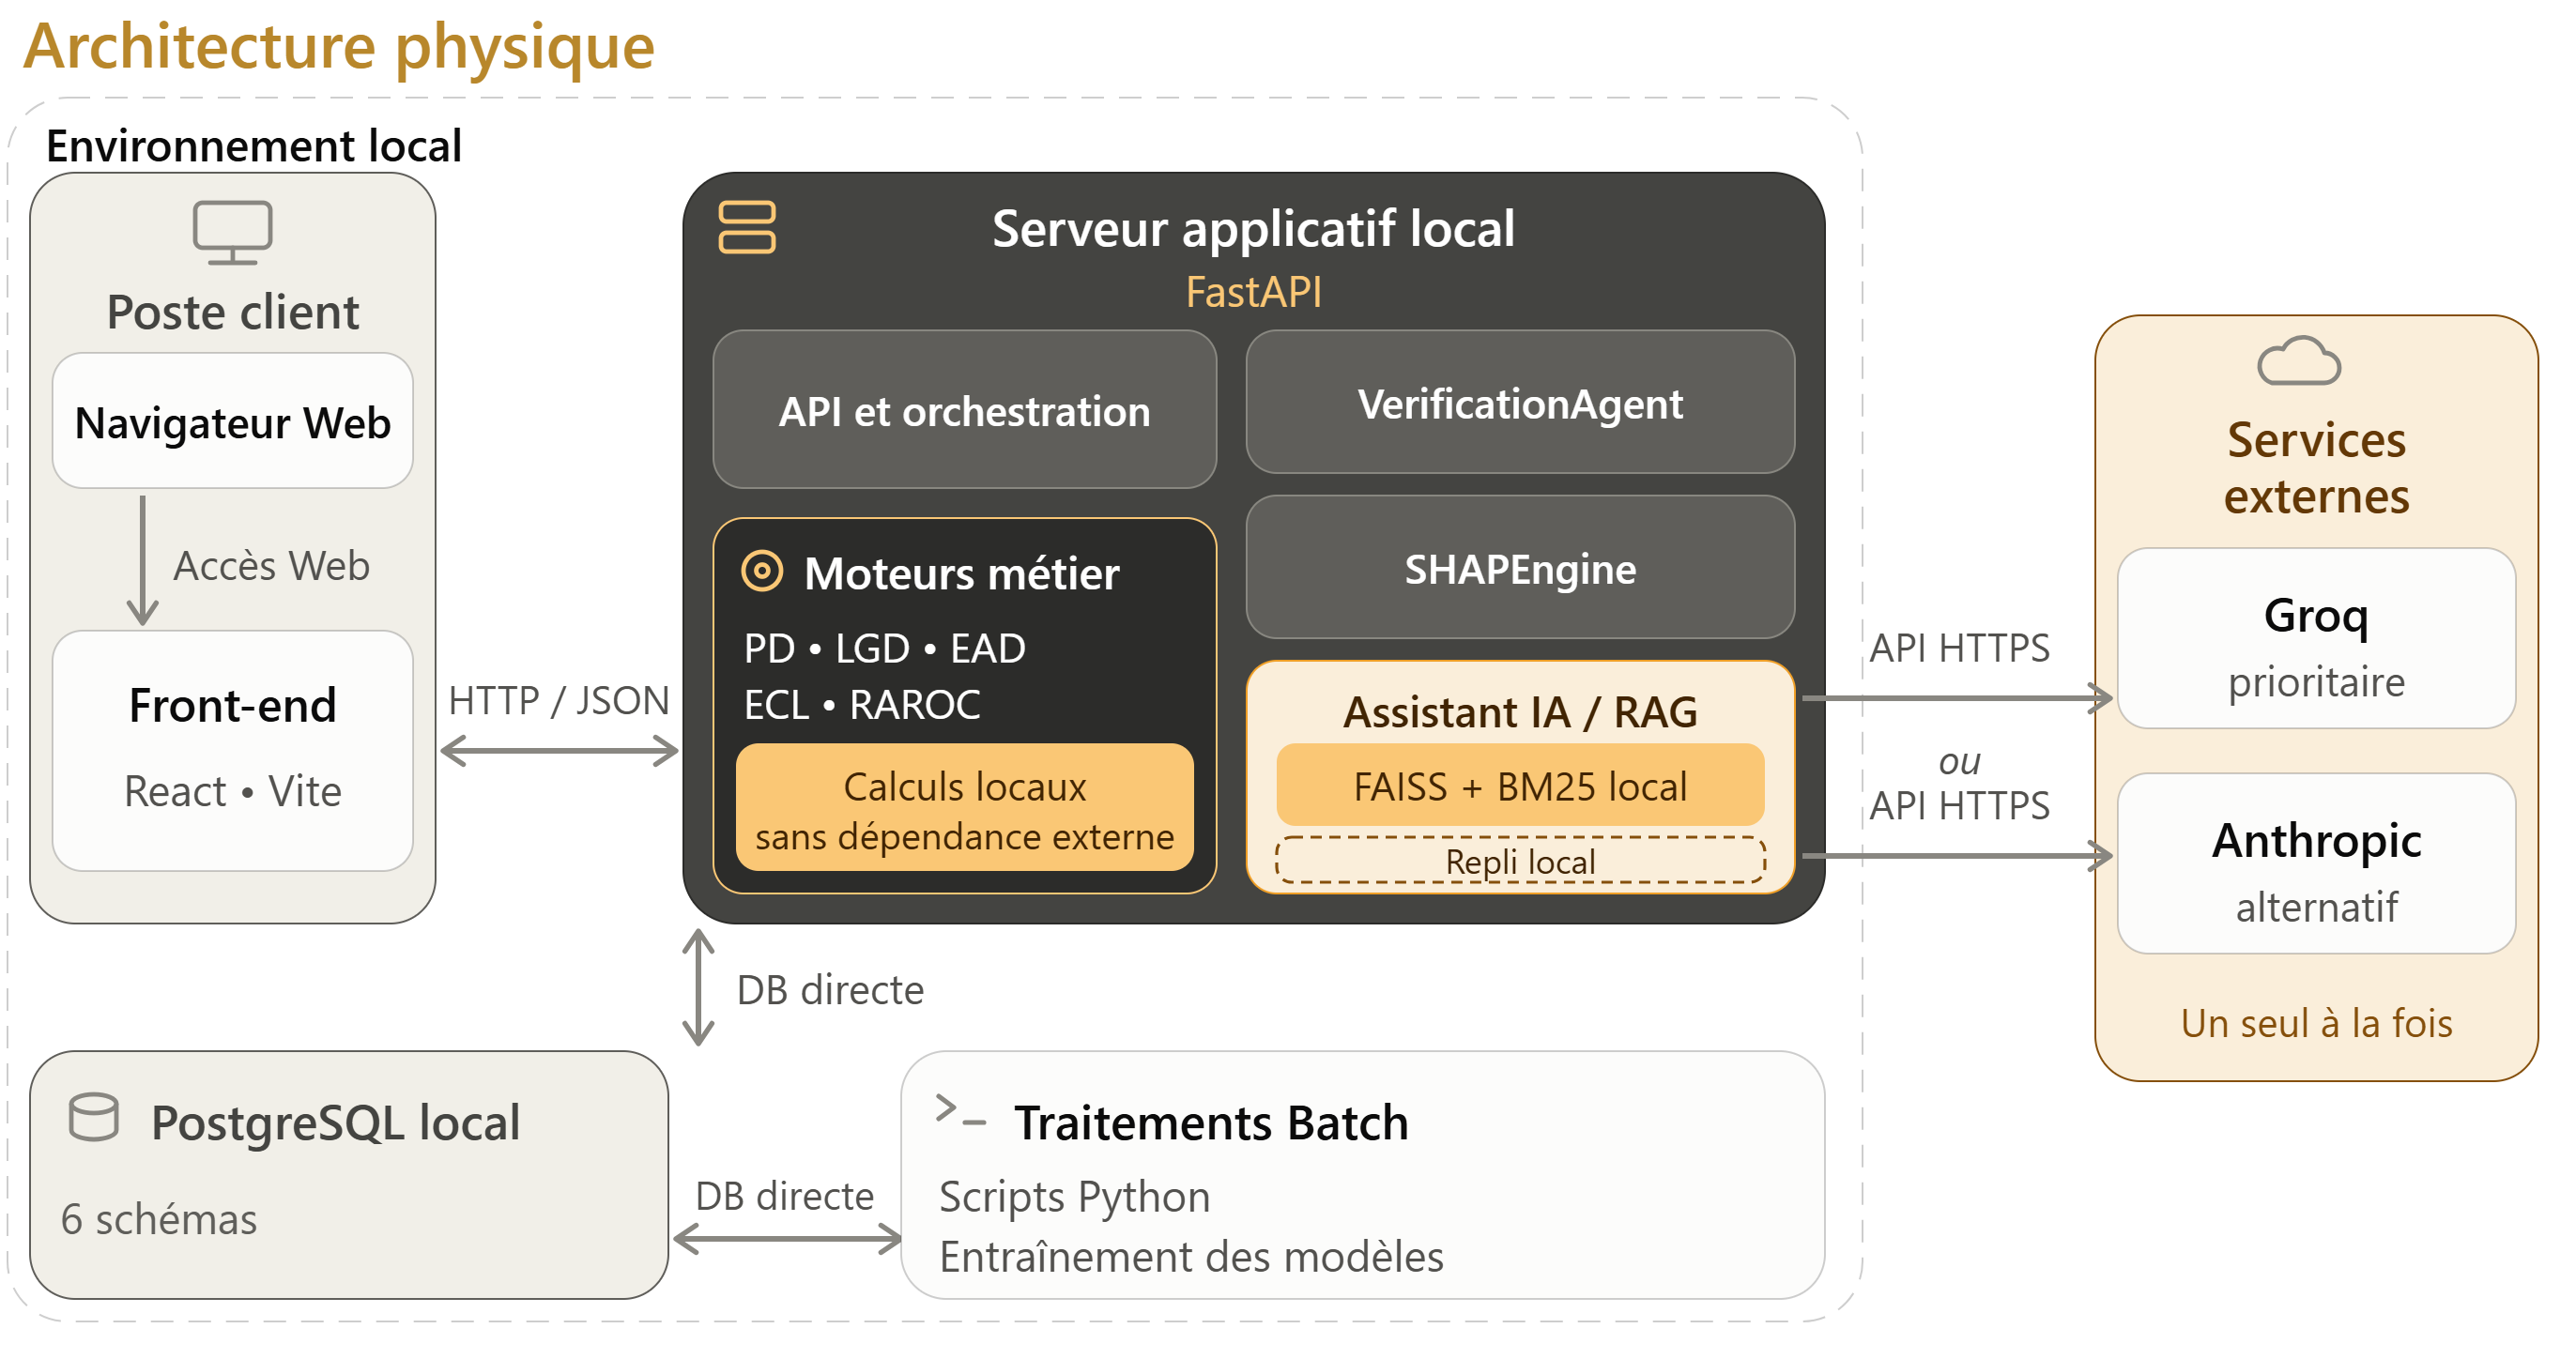
\includegraphics[width=\textwidth]{figures/architecture_physique.png}
    \caption{Architecture physique de la plateforme (élaboration personnelle).}
    \label{fig:architecture-physique}
\end{figure}

Le poste client accède à la plateforme par un navigateur web, qui charge une application front-end développée en React (version 18.3.1) à l'aide de l'outil de développement Vite (version 5.4), servie localement sur le port 5173. Cette application communique avec le serveur applicatif par des requêtes HTTP/JSON, relayées vers le port 8000 par un mécanisme de proxy.

Le serveur applicatif local, un backend FastAPI exécuté par le serveur Uvicorn, regroupe plusieurs composants. Les routes de l'API, les services métier et l'authentification par rôle orchestrent les traitements. Les moteurs de calcul du risque, de rentabilité et de décision, présentés aux chapitres 3 et 4, probabilité de défaut, perte en cas de défaut, exposition au défaut, perte attendue, rentabilité et moteur de décision, s'exécutent localement, sans dépendance à un service externe. Un pipeline d'extraction documentaire, pour l'OCR des documents soumis lors d'une demande, ainsi que le moteur d'interprétabilité SHAP, complètent ce serveur. L'assistant conversationnel, détaillé en section~5.5, s'appuie sur une recherche hybride locale, combinant un index FAISS chargé en mémoire et une recherche lexicale BM25, avant de faire appel à un fournisseur externe de génération de texte : Groq en priorité, ou Anthropic lorsque Groq n'est pas disponible à l'initialisation, un seul des deux étant utilisé à la fois selon cette disponibilité, avec un repli local déterministe si aucun des deux n'est disponible.

Le serveur applicatif et les traitements batch, des scripts Python mobilisant les bibliothèques scikit-learn, XGBoost, LightGBM, SHAP et Optuna déjà présentées au chapitre 3, se connectent tous deux directement à la même base PostgreSQL locale, organisée selon les schémas présentés en section~5.1.

\section{Conception du système et diagrammes UML}

\subsection{Diagramme de séquence du parcours Origination}

La figure~\ref{fig:sequence-origination} détaille, sous la forme d'un diagramme de séquence, l'enchaînement réel des appels pour une demande de crédit, de sa création à sa décision, en deux étapes distinctes.

\begin{figure}[htbp]
    \centering
    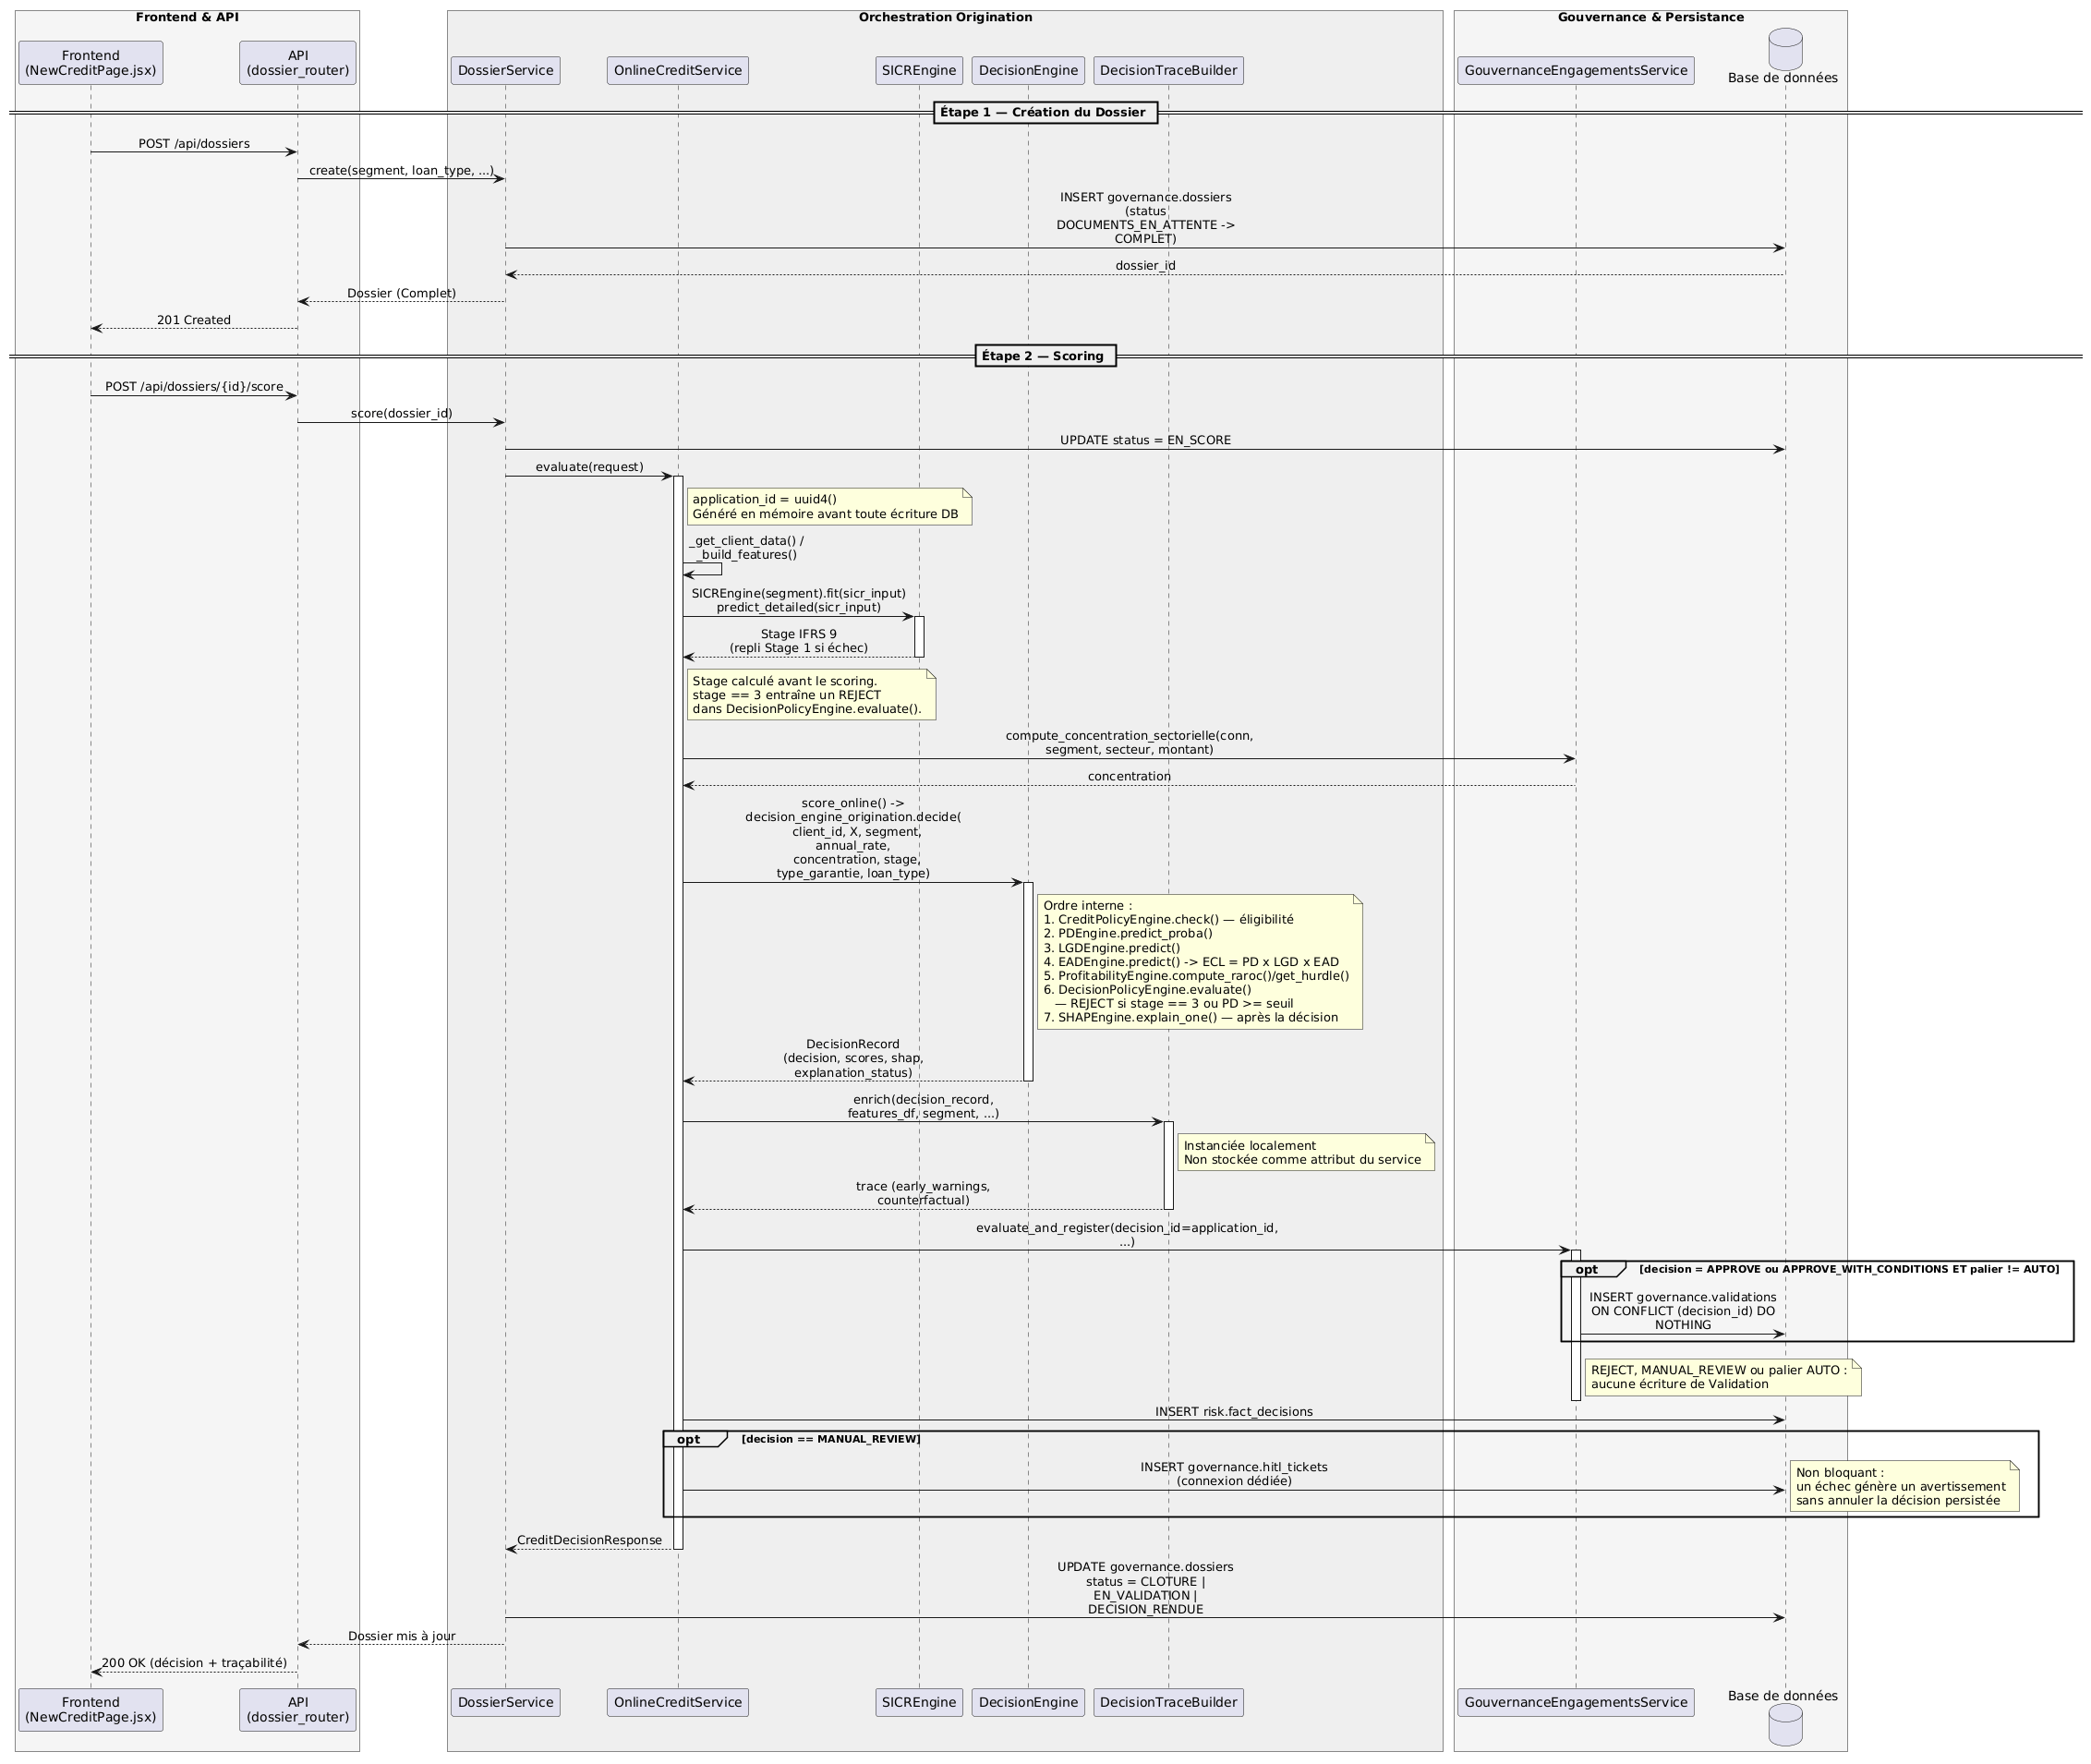
\includegraphics[width=\textwidth]{figures/sequence_origination.png}
    \caption{Diagramme de séquence du parcours Origination (élaboration personnelle).}
    \label{fig:sequence-origination}
\end{figure}

La création du dossier enregistre la demande dans le schéma de gouvernance, dans un statut initial qui évolue une fois les données nécessaires réunies. Le scoring, déclenché séparément, délègue l'ensemble du calcul métier à un point d'entrée unique : un identifiant d'application (\texttt{application\_id}) est généré en mémoire avant la persistance des résultats du scoring, puis le stage IFRS 9 du client est déterminé en amont du scoring, selon les mêmes règles SICR que celles présentées en section~4.2. Ce stage intervient dans l'appréciation de la situation du dossier et dans les règles de décision, sans modifier le calcul simplifié de l'ECL utilisé dans ce parcours, qui repose, pour rappel, sur une probabilité de défaut à douze mois. Le moteur de décision dédié à l'Origination, présenté en section~4.5, est alors invoqué selon l'enchaînement déjà détaillé : éligibilité, probabilité de défaut, perte en cas de défaut, exposition et perte attendue, rentabilité, règles de décision, puis explication SHAP. La décision obtenue est enrichie d'éléments de traçabilité complémentaires, construits à la demande plutôt que conservés en mémoire d'un appel à l'autre, puis soumise à la gouvernance des engagements : une validation humaine n'est enregistrée que si la décision le justifie et que le palier de délégation applicable l'exige, les autres cas n'entraînant aucune écriture à ce titre. Une décision orientée vers une revue manuelle crée, en complément, un ticket dans la file de travail des analystes, sans jamais faire échouer la réponse si cette création rencontre un problème. Le dossier est enfin mis à jour dans un statut qui reflète l'issue de ce traitement.

\subsection{Diagramme de séquence du traitement batch du portefeuille}

La figure~\ref{fig:sequence-monitoring} détaille, sous la forme d'un diagramme de séquence, l'enchaînement réel du traitement batch qui produit un instantané du suivi de portefeuille, pour un mois d'activité donné.

\begin{figure}[htbp]
    \centering
    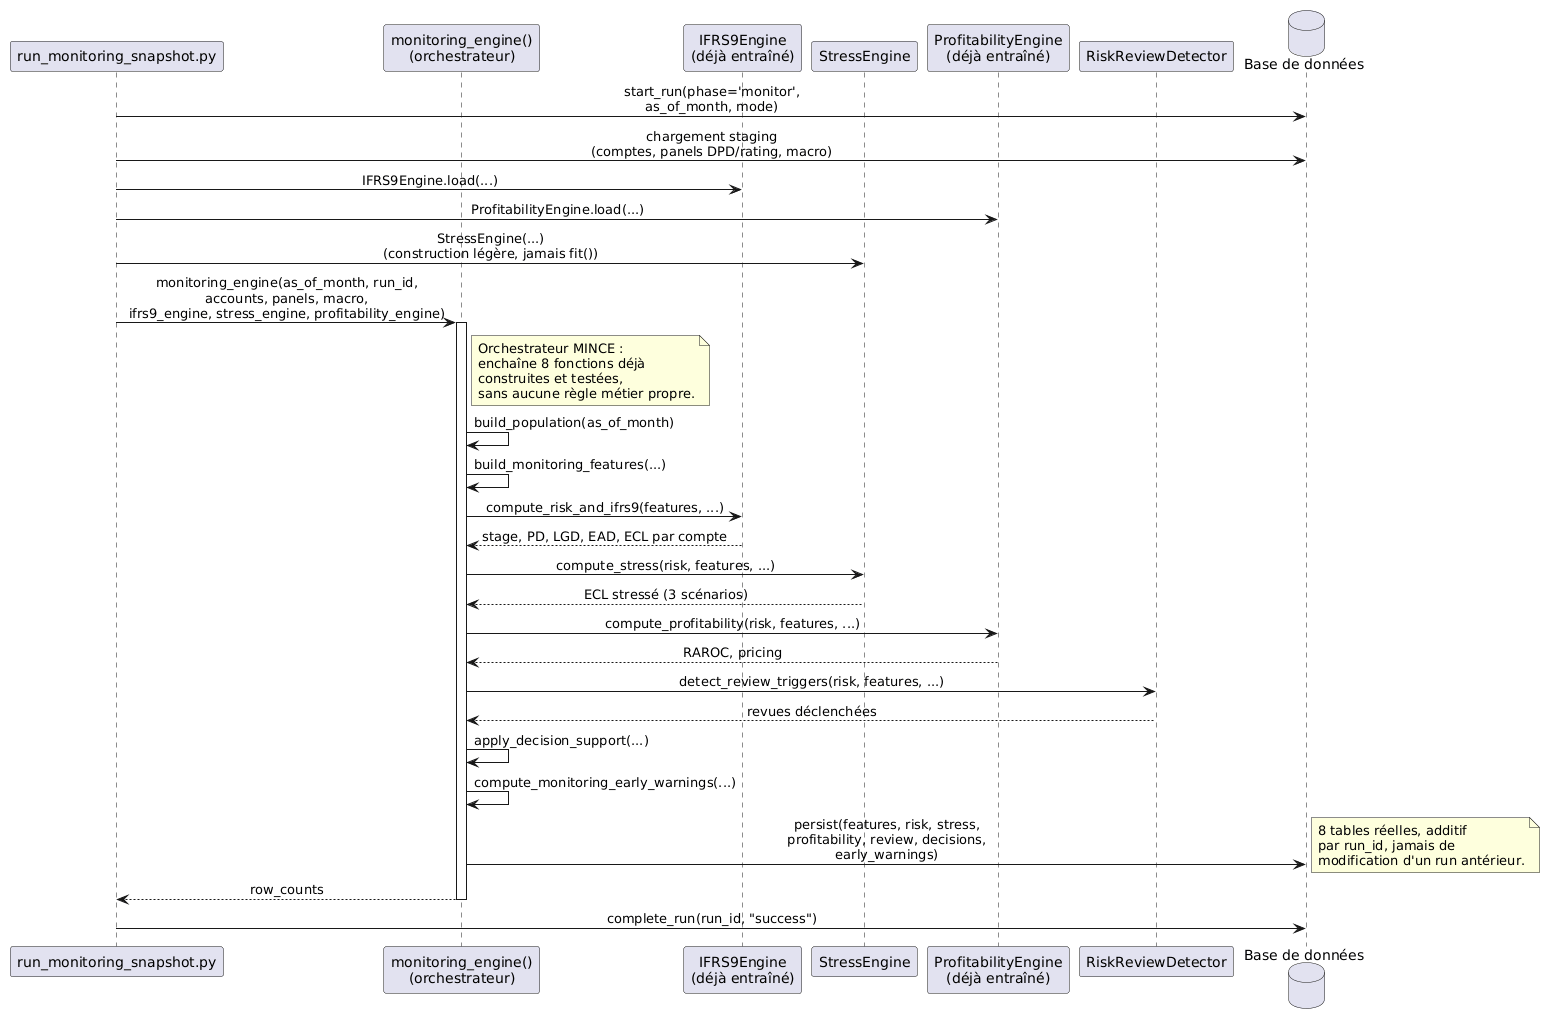
\includegraphics[width=\textwidth]{figures/sequence_monitoring_batch.png}
    \caption{Diagramme de séquence du traitement batch du portefeuille (élaboration personnelle).}
    \label{fig:sequence-monitoring}
\end{figure}

Ce traitement charge d'abord les modèles déjà entraînés, présentés au chapitre 3, ainsi que les données réelles du portefeuille à la date considérée, avant de déléguer l'ensemble du calcul à un orchestrateur unique. Celui-ci enchaîne, dans un ordre fixe, huit étapes déjà construites indépendamment les unes des autres, sans ajouter de règle métier qui lui serait propre : la construction de la population de comptes concernés, la construction des caractéristiques nécessaires, le calcul du risque et des pertes attendues selon IFRS 9, le calcul des indicateurs sous stress, le calcul de la rentabilité, la détection des comptes nécessitant une revue, l'application des règles de suivi du portefeuille, distinctes du moteur de décision d'Origination présenté ci-dessus, puis le calcul de signaux de vigilance complémentaires. Le résultat de ces huit étapes est enfin persisté dans les tables réelles du suivi de portefeuille, de façon additive par exécution, sans jamais modifier une exécution antérieure.

\subsection{Diagramme d'activité du processus de décision}

La figure~\ref{fig:activite-decision} représente, sous la forme d'un diagramme d'activité, l'enchaînement des règles hiérarchiques présentées en section~4.5, depuis la vérification de l'éligibilité jusqu'à l'une des quatre catégories de décision possibles.

\begin{figure}[htbp]
    \centering
    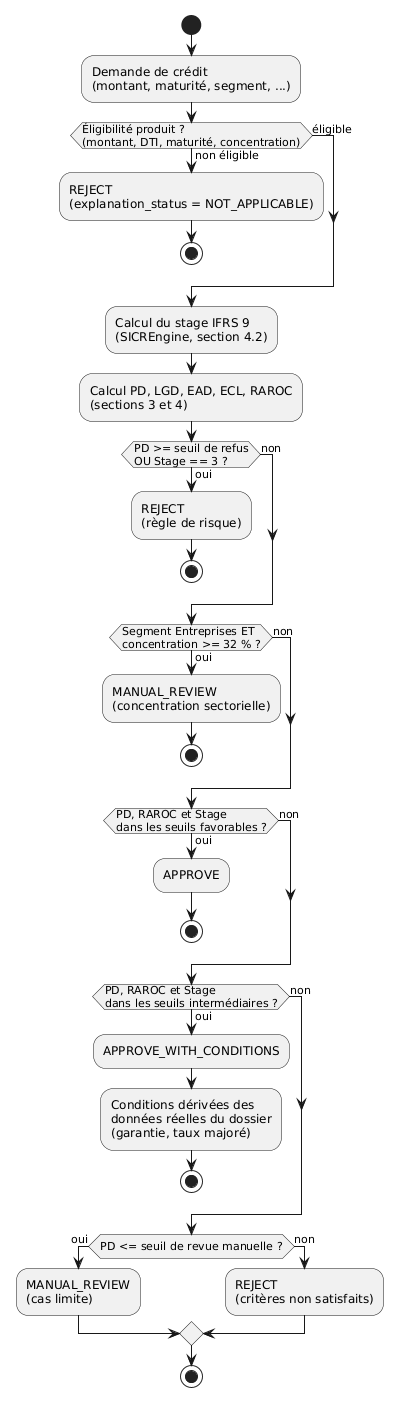
\includegraphics[width=\textwidth,height=0.85\textheight,keepaspectratio]{figures/activite_decision_origination.png}
    \caption{Diagramme d'activité du processus de décision Origination (élaboration personnelle).}
    \label{fig:activite-decision}
\end{figure}

Ce diagramme met en évidence deux propriétés déjà soulignées au chapitre 4 : l'éligibilité est vérifiée avant tout calcul de risque, de sorte qu'un refus à ce stade n'engage jamais les modèles prédictifs ; et les règles de décision proprement dites s'appliquent ensuite dans un ordre strictement hiérarchique, un refus fondé sur le risque ou le stage prévalant sur toute autre règle, jusqu'au cas limite qui bascule vers une revue manuelle plutôt que vers un refus automatique.

\subsection{Diagramme de classes}

La figure~\ref{fig:diagramme-classes} présente l'organisation des classes qui implémentent les moteurs métier et leur orchestration.

\begin{figure}[htbp]
    \centering
    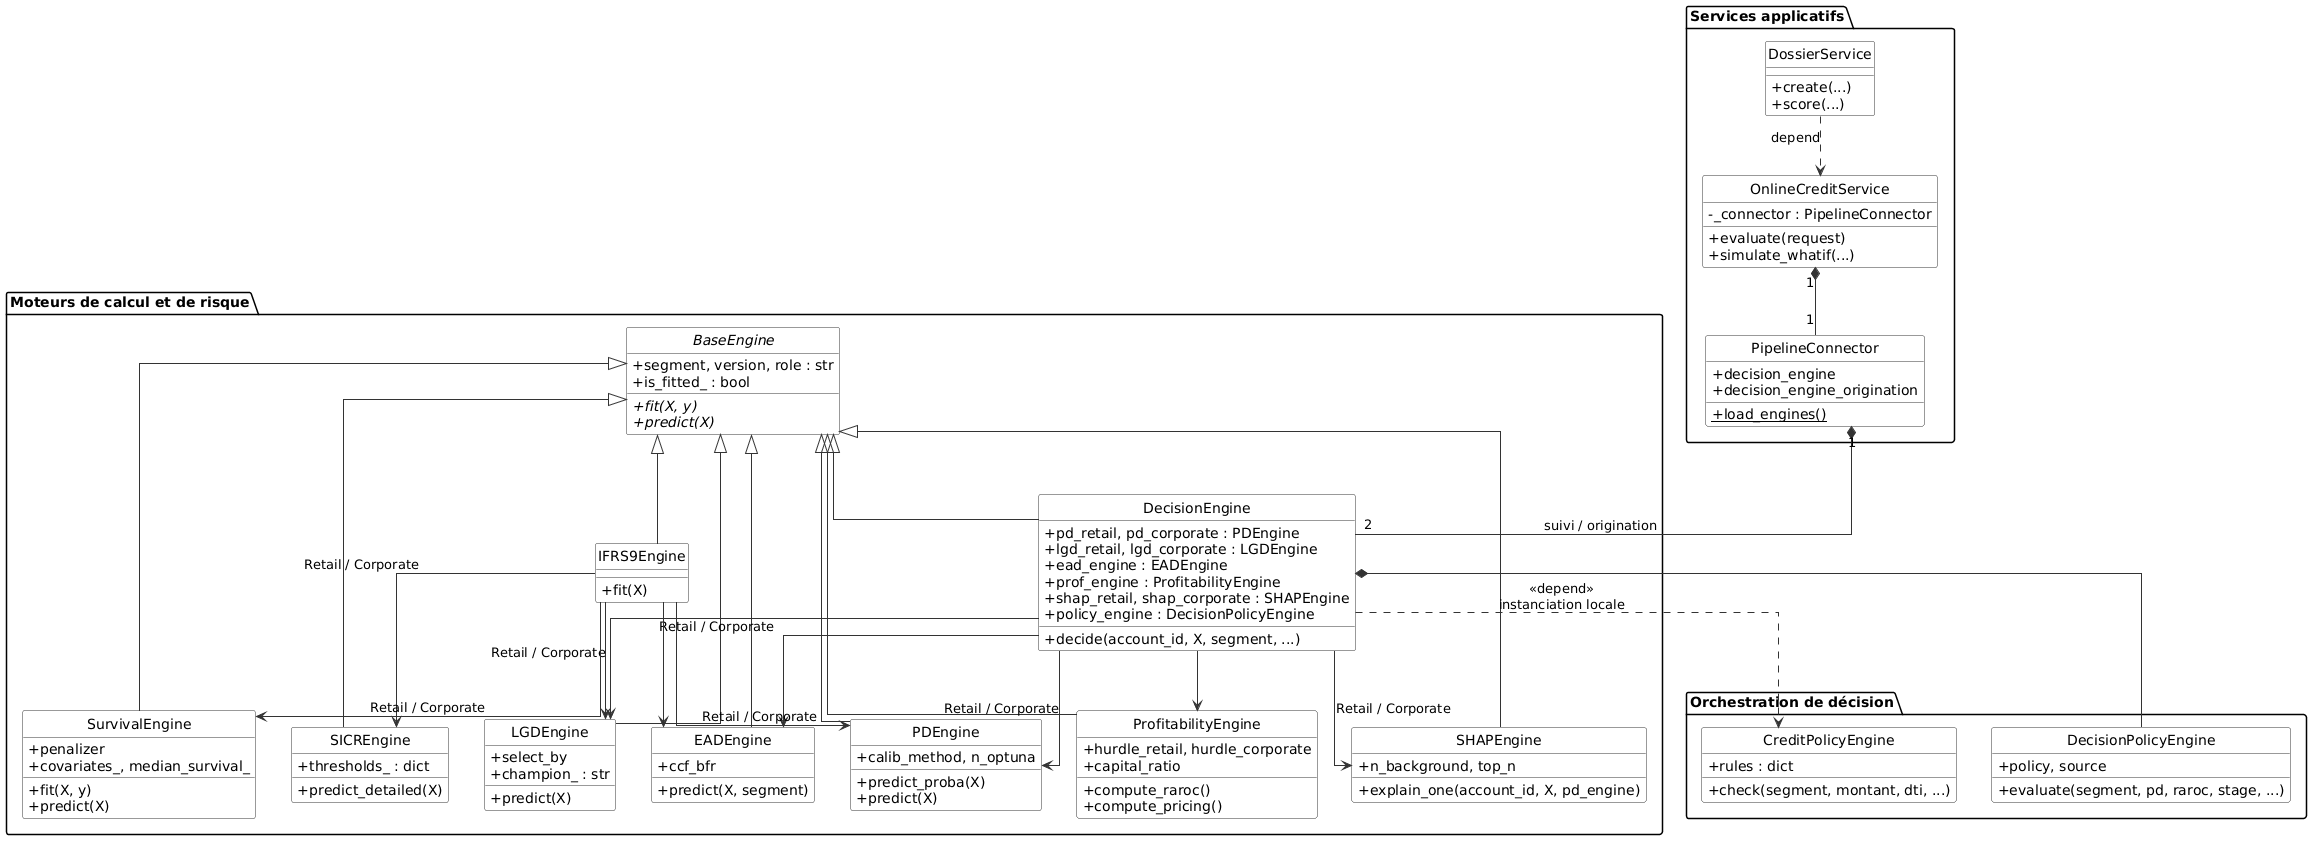
\includegraphics[width=\textwidth]{figures/diagramme_classes.png}
    \caption{Diagramme de classes des moteurs de calcul et de décision (élaboration personnelle).}
    \label{fig:diagramme-classes}
\end{figure}

L'ensemble des moteurs de risque présentés aux chapitres 3 et 4, probabilité de défaut, perte en cas de défaut, exposition au défaut, détection de dégradation du risque, modèle de survie, rentabilité et interprétabilité SHAP, hérite d'une classe commune qui définit leur interface : des attributs partagés (segment, version, rôle), un indicateur d'état entraîné, et deux méthodes de même signature, l'une pour la préparation du moteur, l'autre pour le calcul de sa sortie. Cette interface commune ne signifie pas que chaque moteur apprend statistiquement à partir de données : pour l'exposition au défaut ou la détection de dégradation du risque, présentées comme des formules déterministes aux chapitres 3 et 4, la méthode de préparation ne fait que valider les données attendues, sans ajustement de paramètres. Le moteur qui orchestre le calcul des pertes attendues selon IFRS 9, présenté en section~4.2, hérite de cette même classe et compose plusieurs de ces moteurs.

Le moteur de décision, présenté en section~4.5, compose à son tour les moteurs de probabilité de défaut, de perte en cas de défaut, d'exposition au défaut, de rentabilité et d'interprétabilité SHAP, distinctement pour chaque segment, ainsi qu'un moteur de règles de décision et un moteur d'éligibilité, présentés eux aussi en section~4.5. Conformément à la distinction établie en section~5.1, deux instances de ce moteur de décision coexistent, l'une pour le suivi de portefeuille, l'autre dédiée à l'Origination ; le connecteur qui charge les artefacts entraînés en conserve une référence distincte pour chacune, et c'est exclusivement celle dédiée à l'Origination que mobilise le service de crédit en ligne, lui-même sollicité par le service de gestion des dossiers présenté dans le diagramme de séquence précédent.

\section{Architecture de l'assistant IA}

L'assistant conversationnel déjà introduit en section~5.1 interroge les données et résultats déjà produits par la plateforme, sans jamais calculer lui-même un indicateur de risque ni intervenir dans une décision de crédit ; cette limite est imposée dans le code, par un message rappelé à chaque réponse, et non seulement documentée. Son architecture s'organise en plusieurs étapes.

\begin{figure}[H]
\centering
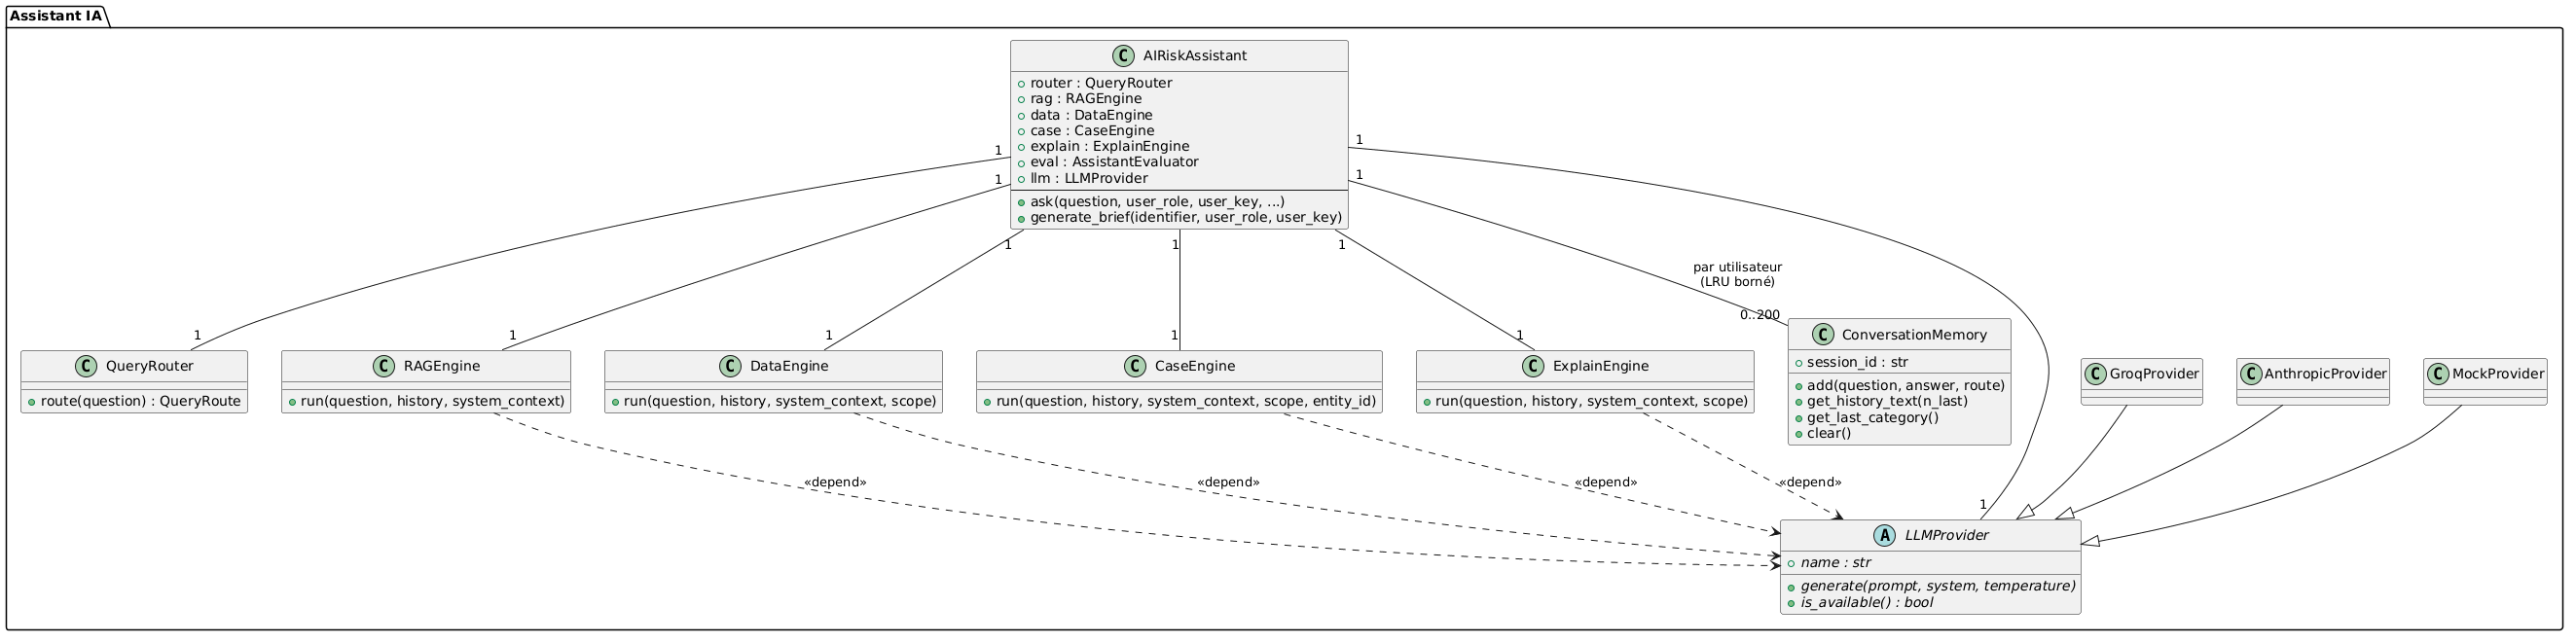
\includegraphics[width=\textwidth]{figures/diagramme_classes_assistant.png}
\caption{Diagramme de classes du sous-système Assistant IA}
\label{fig:diagramme-classes-assistant}
\end{figure}

La figure~\ref{fig:diagramme-classes-assistant} complète le diagramme de classes des moteurs de risque et de l'orchestration de décision présenté en section~5.4 : \texttt{AIRiskAssistant} orchestre un routeur et quatre moteurs spécialisés, partage un même fournisseur de génération de texte, interchangeable sans modifier le code appelant, et gère une mémoire conversationnelle par utilisateur authentifié, bornée par éviction LRU plutôt qu'une instance unique partagée.

Une question posée en langage naturel est d'abord orientée vers l'un de quatre moteurs spécialisés par un routeur à deux niveaux : une première couche de mots-clés traite rapidement les cas évidents, une seconde couche, fondée sur la similarité sémantique entre la question et des exemples de référence, traite les cas plus ambigus. Les questions portant sur la réglementation ou des notions générales (IFRS 9, BCEAO) sont dirigées vers un moteur de recherche documentaire ; celles portant sur le portefeuille, vers un moteur interrogeant directement les résultats déjà calculés ; celles portant sur un dossier client particulier, vers un moteur dédié ; celles portant sur l'interprétation d'un résultat, vers un moteur d'explication s'appuyant sur les valeurs SHAP présentées au chapitre 3.

Le moteur de recherche documentaire repose sur une recherche hybride locale, déjà présentée en section~5.3 : un index FAISS d'embeddings sémantiques, combiné à une recherche lexicale BM25, afin de retrouver les passages pertinents d'une base documentaire réglementaire. Les passages documentaires retrouvés ou les résultats fournis par les moteurs spécialisés constituent le contexte transmis au fournisseur de génération de texte. Celui-ci les exploite pour formuler une réponse en langage naturel, sans se substituer aux moteurs qui produisent les données et les indicateurs.

Le contrôle d'accès par rôle, présenté au chapitre 2, s'applique à deux niveaux distincts avant qu'une donnée n'atteigne ce fournisseur externe. D'abord, à l'intérieur même des moteurs spécialisés, chaque résultat de requête est filtré selon les catégories de données autorisées pour le rôle de l'utilisateur, probabilité de défaut, perte en cas de défaut, exposition, perte attendue, rentabilité, facteurs SHAP, décisions ou revues, un chargé de clientèle n'obtenant par exemple jamais les catégories de risque quantitatif réservées à un analyste crédit ou à un Risk Manager. Un second contrôle, appliqué au texte de contexte assemblé, complète ce filtrage avant la transmission au fournisseur externe. Cette double frontière vise à empêcher qu'une donnée non autorisée pour un rôle n'entre dans le contexte transmis au fournisseur de génération, plutôt que de compter sur ce dernier pour ne pas la restituer.

Une mémoire conversationnelle, propre à chaque utilisateur authentifié, conserve les derniers échanges afin de résoudre les références d'une question à l'autre, par exemple « son RAROC », en référence au dernier client mentionné. Avant sa restitution, chaque réponse fait également l'objet d'une auto-évaluation, un contrôle supplémentaire sur la réponse produite, qui ne constitue ni une validation humaine ni une preuve de son exactitude. Enfin, les échanges sont soumis à une double traçabilité : un journal propre à l'assistant et le journal d'audit chaîné de la plateforme, présenté au chapitre 2.

\begin{figure}[H]
\centering
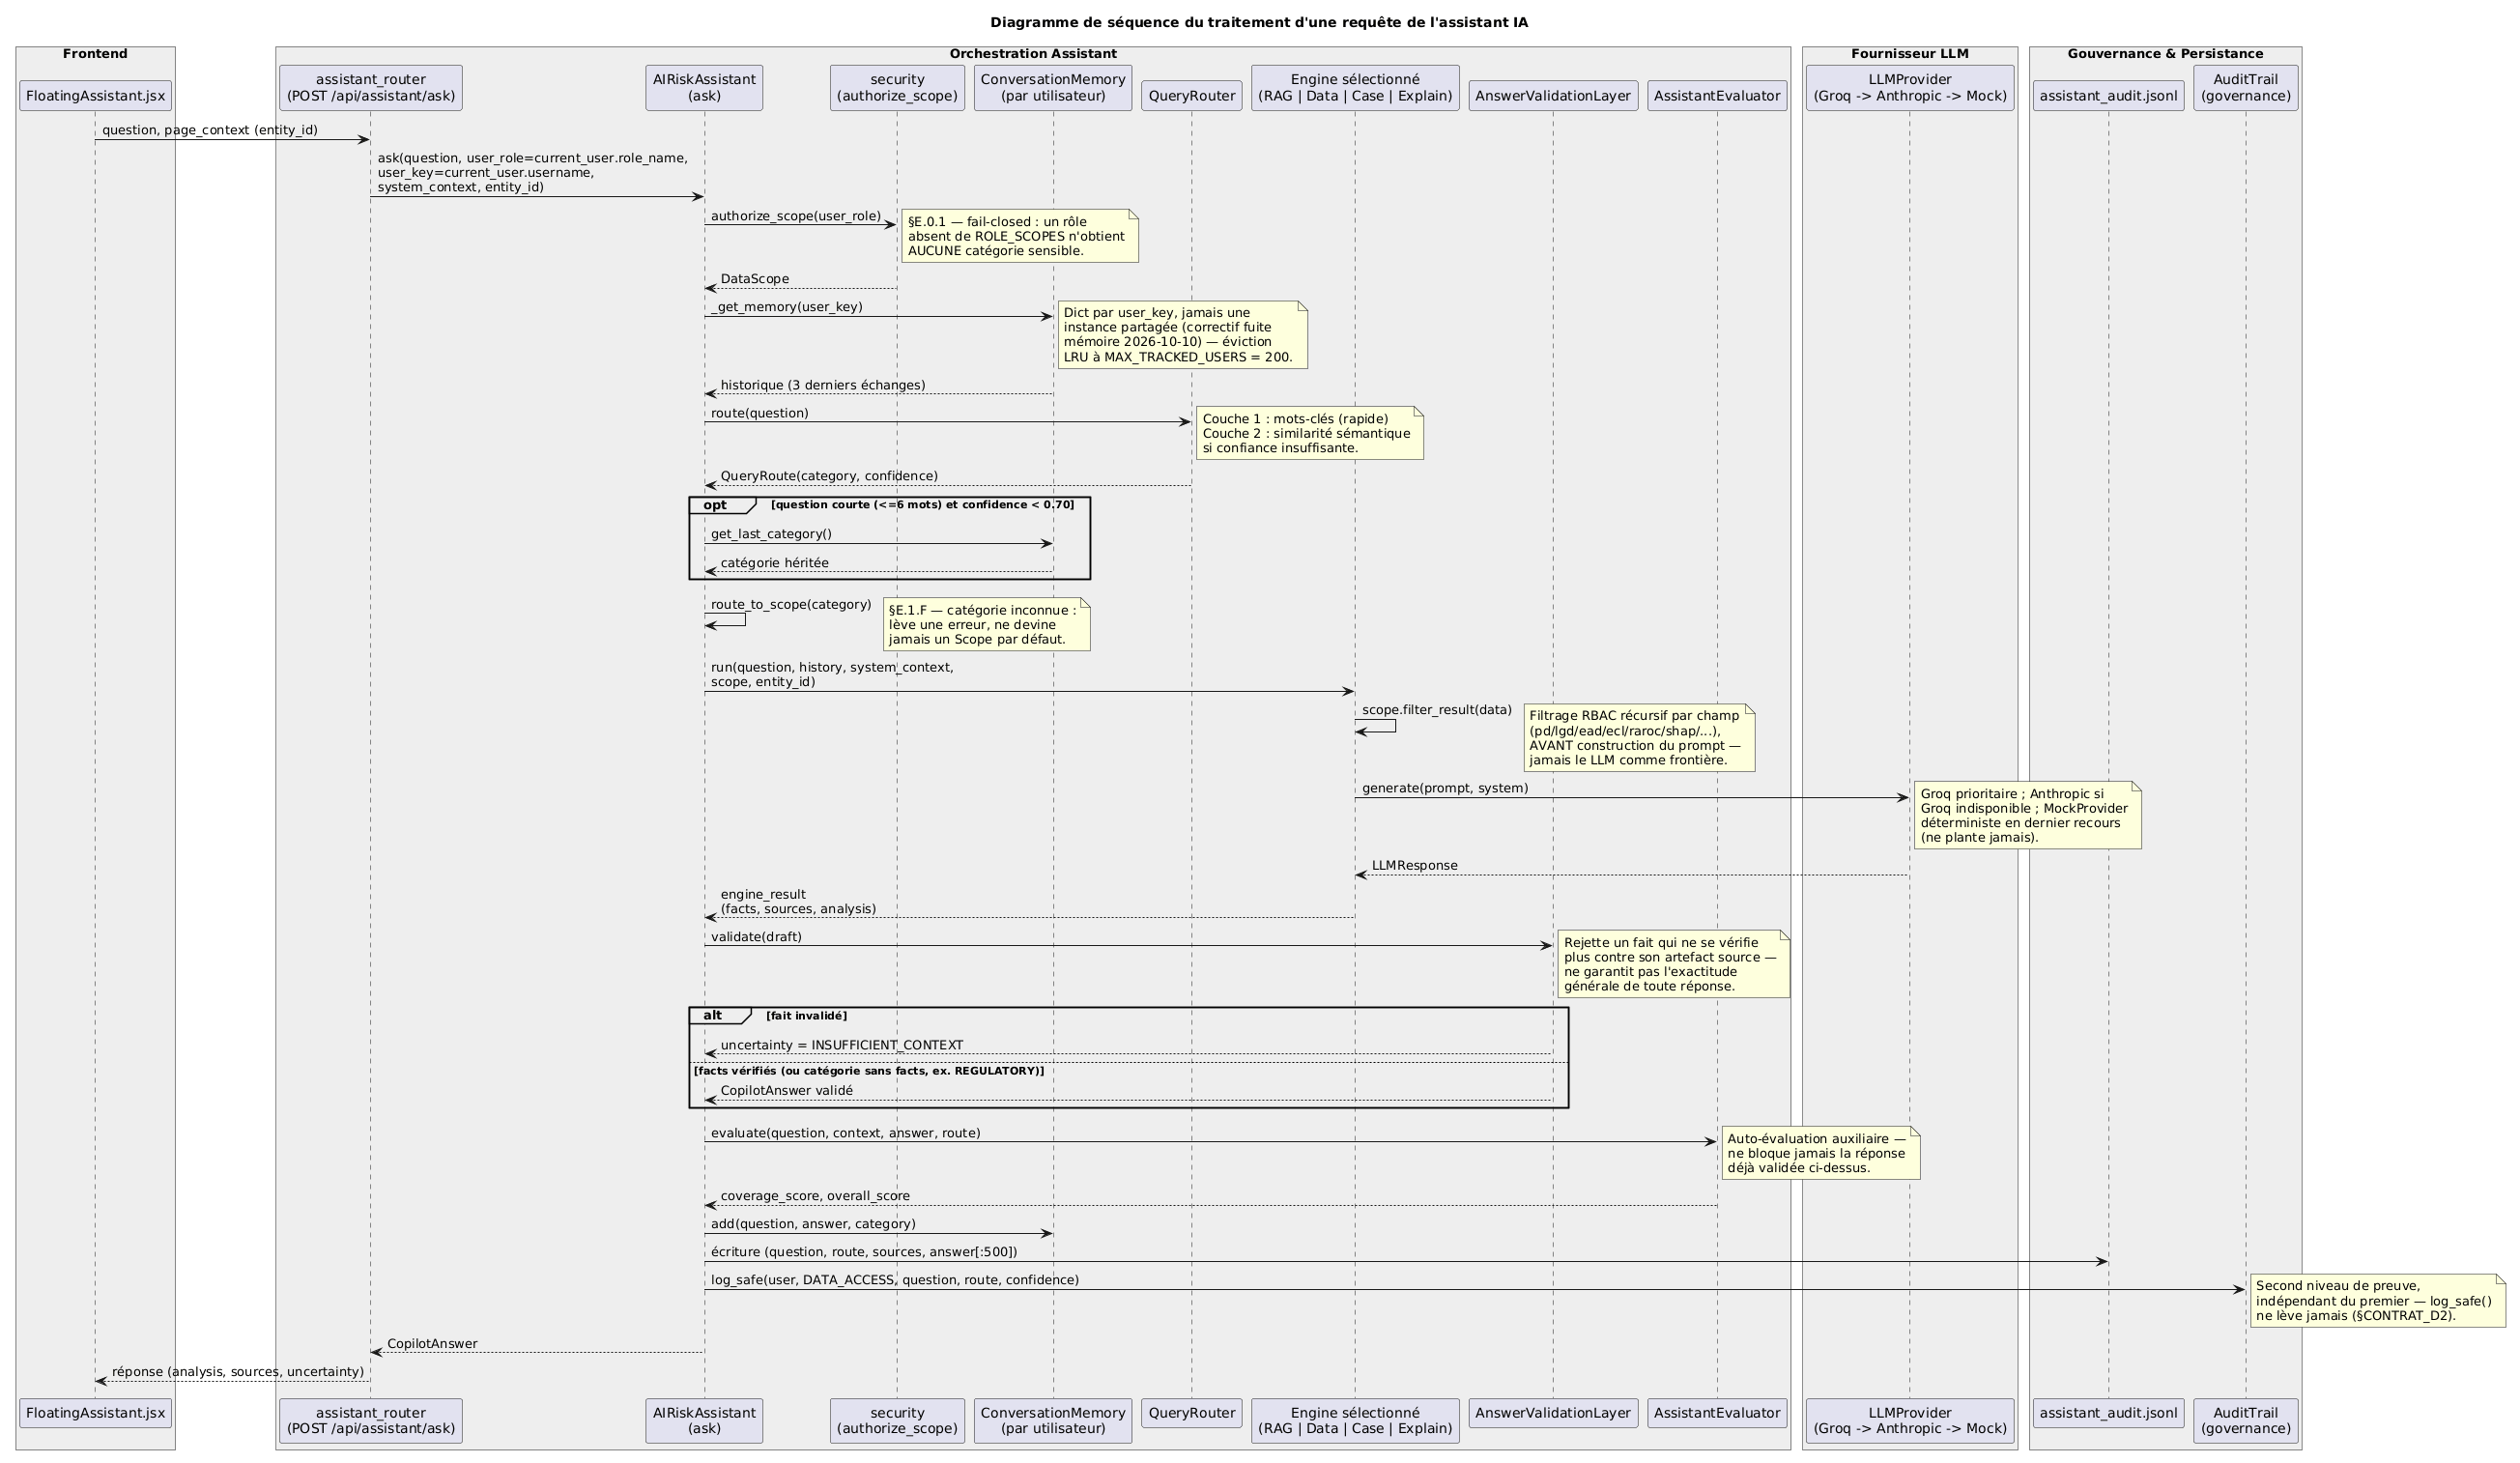
\includegraphics[width=\textwidth]{figures/sequence_assistant.png}
\caption{Diagramme de séquence du traitement d'une requête de l'assistant IA}
\label{fig:sequence-assistant}
\end{figure}

La figure~\ref{fig:sequence-assistant} rend explicite l'ordre réel de ces étapes, déjà décrites en prose ci-dessus : le contrôle d'accès par rôle est résolu avant même la mémoire conversationnelle, le routage attribue un \textit{Scope} explicite qui échoue plutôt que de deviner une catégorie par défaut, et le filtrage RBAC s'exécute à la sortie de chaque moteur spécialisé, avant la construction du prompt transmis au fournisseur externe. La couche de validation des réponses rejette un fait qui ne se vérifie plus contre son artefact source, sans garantir pour autant l'exactitude générale de toute réponse produite ; l'auto-évaluation qui suit reste, de la même façon, un contrôle auxiliaire et non une preuve de correction.

\section*{Conclusion du chapitre}

Ce chapitre a présenté l'architecture qui met en œuvre les modèles et les mécanismes décrits aux chapitres 3 et 4. Deux chemins de traitement, l'un batch, l'autre temps réel, coexistent sans dupliquer toute leur logique : plusieurs moteurs de calcul sont réutilisés entre eux, tandis que d'autres composants, modèles entraînés, moteur de décision effectivement exécuté, restent propres à l'un ou à l'autre. Cette organisation logique repose sur une réalisation technique précise, détaillée par les diagrammes d'architecture et les diagrammes UML présentés, et s'accompagne d'un assistant conversationnel qui complète la plateforme sans jamais se substituer à ses mécanismes de décision, ses propres garde-fous d'accès aux données faisant l'objet d'une attention comparable à celle des moteurs de risque. Le chapitre suivant aborde la réalisation effective de cette architecture et sa mise en œuvre, jusqu'à sa validation.
